\subsection{Misura dello Slew Rate}

\begin{wrapfigure}[16]{r}{0.55\textwidth}
  \begin{center}
    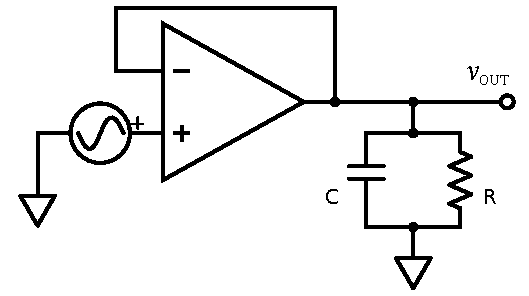
\includegraphics[width=0.30\textwidth]{../E03/latex/slew_rate.pdf}
  \end{center}
  \caption{Schema del circuito utilizzato per stimare lo Slew Rate. La resistenza utilizzata è $R=2.17\pm0.01$\si{\kilo\ohm}; la capacità $C=200 \pm 10$ \si{\pico\farad}.}
  \label{cir2:slew_rate}
\end{wrapfigure}

L'amplificatore operazionale ha una capacità limitata di ricorrere segnali: ciò significa che, data una funzione in entrata nell'OP-AMP, quest'ultimo non sarà in grado di restituire in uscita il segnale amplificato con la stessa forma d'onda. In altre parole, l'amplificatore ha un valore
$$SR = \frac{\Delta V}{\Delta t}$$
costante. Questo fenomeno è dunque visibile a valori di tensione e frequenza che superino lo $SR$.

Nel nostro caso abbiamo utilizzato il generatore, caratterizzato da uno Slew Rate di $SR_{gen}=315$ \si{\volt\per\micro\second}, per creare il segnale in ingresso (onda quadra) e valutato la forma d'onda del segnale in uscita utilizzando il circuito in Figura ????????? quando aveva derivata $dV/dt > 0$. La capacità è utilizzata come serbatoio di cariche per attenuare fenomeni di rumore nel segnale creati dal generatore.

Inizialmente abbiamo posto la frequenza a $f=1$\si{\kilo\hertz} e la tensione picco picco a $V_{pp}=10$ \si{\volt}; con la funzione cursore dell'oscilloscopio abbiamo poi misurato $\Delta V = 8.0719$ \si{\volt} fra il 10\% e il 90\% del valore di tensione picco picco in uscita e la relativa $\Delta t = 15.92$ \si{\micro\second}, ottenendo uno $SR=0.507$ \si{\volt\per\micro\second}.

Come però si può vedere dal grafico in Figura ?????? si nota che nella parte vicina al 10\% è presente una parte di segnale affetta da rumore che potrebbe rendere poco precisa la nostra misura. Infatti siamo interessati al rapporto fra i $\Delta$; dunque portare il limite inferiore ad un valore percentuale più alto, dato il rumore, rende più precisa la misura. Portando dunque la percentuale del limite inferiore al 25\% abbiamo ottenuto i seguenti valori: $\Delta V = 6.4813$ \si{\volt} e $\Delta t = 14.5$ \si{\micro\second}, dunque $SR = 0.447$ \si{\volt\per\micro\second}. Durante l'esperienza utilizzeremo questo valore come riferimento per lo Slew Rate del nostro amplificatore.

Abbiamo anche notato che lo Slew Rate è differente a seconda che il segnale abbia derivata $dV/dt$ positiva o negativa. In questo secondo caso, infatti, abbiamo ottenuto i seguenti valori: $\Delta V = 7.975$ \si{\volt} e $\Delta t = 11.42$ \si{\micro\second}, quindi $SR = 0.698$ \si{\volt\per\micro\second}.